% 2006 年全国卷Ⅱ理科第 7 题：两个互相垂直的平面
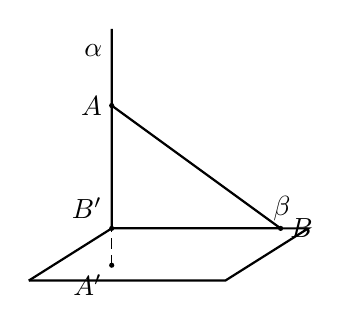
\begin{tikzpicture}[>=stealth,scale=0.78]
  \coordinate (I) at (0,0);
  \coordinate (J) at (1.35,0.85);
  \coordinate (K) at (4.55,0.85);
  \coordinate (L) at (3.20,0);
  \coordinate (Atop) at (1.35,4.10);
  \coordinate (A) at (1.35,2.85);
  \coordinate (Aprime) at (1.35,0.25);
  \coordinate (Bprime) at (1.35,0.85);
  \coordinate (B) at (4.10,0.85);
  \draw[thick] (I)--(J)--(Atop);
  \draw[thick] (I)--(L)--(K)--(J);
  \draw[thick] (J)--(B);
  \draw[thick] (A)--(B);
  \draw[dashed] (A)--(Aprime) (Aprime)--(Bprime);
  \fill (A) circle (1.2pt) node[left] {$A$};
  \fill (Aprime) circle (1.2pt) node[below left] {$A'$};
  \fill (Bprime) circle (1.2pt) node[above left] {$B'$};
  \fill (B) circle (1.2pt) node[right] {$B$};
  \node at (1.05,3.75) {$\alpha$};
  \node at (4.12,1.18) {$\beta$};
\end{tikzpicture}
